
\section{Effective constructions} \label{s:effective constructions}	

In this section we construct explicit May-Steenrod structures on three well know combinatorial $E_\infty$-operads: the Barratt-Eccles operad $\mathcal E$ \cite{berger04combinatorial}, the surjection operad $\mathcal X$ \cite{mcclure03cochain}, and the operad $U(\mathcal M)$ associated to the finitely presented $E_\infty$-PROP $\mathcal M$ \cite{medina2020prop1}. We also define natural and effective May-Steenrod structure on the normalized cochains of any simplicial or cubical set, by describing a $U(\mathcal M)$-algebra structures on it.

Figure~\ref{fig: bigsummary} presents a diagrammatical representation of the constructions in this section.

\begin{figure}
	\begin{tikzcd}
	& & & U(\mathcal M) \arrow[dddr, bend left=10, "\phi^\triangle"'] \arrow[dddrr, bend left=20, "\phi^\square"'] & & \\
	& & \mathcal X \arrow[ru, "SL"] & & & \\
	& \mathcal E \arrow[ur, "TR"] & & & & \\
	\mathcal W \arrow[rrrr, "\psi^\triangle", bend right=10] \arrow[rrrrr, "\psi^\square", bend right=20] \arrow[ur, "\psi_{\mathcal E}"] \arrow[uurr, "\psi_{\mathcal X}"', bend right=35, pos=.6] \arrow[uuurrr, "\psi_{U(\mathcal M)}"', bend right=45, pos=0.6] & & & & \End_{N^\bullet(X)} & \End_{N^\bullet(X)}
	\end{tikzcd}
	\caption{Summary of effective constructions: May-Steenrod structures on the Barratt-Eccles $\mathcal E$, surjection $\mathcal X$, and $U(\mathcal M)$ operads, and natural May-Steenrod structures on the normalized chains of simplicial and cubical sets. We are abusing notation since the maps $TR$ and $SL$ required different sign conventions.}
	\label{fig: bigsummary}
\end{figure}

\subsection{Barratt-Eccles operad} In this subsection we effectively describe a May-Steenrod structure on the Barratt-Eccles operad.

We begin by reviewing the $\mathrm{S}$-module structure underlying the Barratt-Eccles operad and, since will not use it in this work, refer to \cite{berger04combinatorial} for a description of if composition structure. For a non-negative integer $r$ define the simplicial set $E(\mathrm S_r)$ by 
\begin{equation} \label{eq: milnor model of symmetric}
\begin{split}
E(\mathrm S_r)_n &= \{ (\sigma_0, \dots, \sigma_n)\ |\ \sigma_i \in \mathrm{S}_r\}, \\
d_i(\sigma_0, \dots, \sigma_n) &= (\sigma_0, \dots, \widehat{\sigma}_i, \dots, \sigma_n), \\
s_i(\sigma_0, \dots, \sigma_n) &= (\sigma_0, \dots, \sigma_i, \sigma_i, \dots, \sigma_n) \\
\end{split}
\end{equation}
with a left $\mathrm S_r$-action given by
\begin{equation*}
\sigma (\sigma_0, \dots, \sigma_n) = (\sigma \sigma_0, \dots, \sigma \sigma_n).
\end{equation*} 
The chain complex resulting from applying the functor of normalized integral chains to it is denoted $\mathcal E(r)$, which corresponds to the arity $r$ part of the Barratt-Eccles operad.

\begin{definition} \label{def: Steenrod-Adem on Barratt-Eccles}
	For every $r \geq 0$, let $\psi_{\mathcal E}(r) : \mathcal W(r) \to \mathcal E(r)$ be the $\Z[\mathrm{C}_r]$-linear map defined on basis elements by 
	\begin{equation*}
	\psi_{\mathcal E}(r)(e_{n}) = \begin{cases}
	\displaystyle{\sum_{r_1, \dots, r_m}} \big(\rho^0, \rho^{r_1}, \rho^{r_1+1}, \rho^{r_2}, \dots, \rho^{r_{m}}, \rho^{r_{m}+1} \big) & n = 2m, \\
	\displaystyle{\sum_{r_1, \dots, r_m}} \big(\rho^0, \rho^1, \rho^{r_1}, \rho^{r_1+1}, \dots, \rho^{r_{m}}, \rho^{r_{m}+1} \big) & n = 2m+1,
	\end{cases}
	\end{equation*}
	where the sum is over all $r_1, \dots, r_m \in \{0, \dots, r-1\}$.
\end{definition}

\begin{theorem} \label{thm: Steenrod-Adem on Barratt-Eccles}
	The morphism of $\mathrm{C}$-modules
	\begin{equation*}
	\psi_{\mathcal E} \colon \mathcal W \to \mathcal E
	\end{equation*}
	defines a May-Steenrod structure on the Barratt-Eccles operad.
\end{theorem}

\begin{proof}
	This theorem follows from a computation which we defer to the appendix.
\end{proof}

\begin{example}
	Table \ref{fig: Barratt-Eccles Steenrod products} shows $\psi_{\mathcal E}(r)(e_n)$ for small values of $r$ and $n$.
\end{example}

\begin{table}[h]
	\centering
	\resizebox{0.8\columnwidth}{!}{%
		\renewcommand{\arraystretch}{1.2}
		\begin{tabular}{|c||c|c|c|}
			\hline
			$r$ & $n=2$ & $n=3$ & $n=4$ \\
			\hline
			2 & (0,1,0) & (0,1,0,1) & (0,1,0,1,0) \\
			\hline
			3 & (0,1,2) + (0,2,0) & (0,1,2,0) + (0,1,0,1) & \phantom{+} (0,1,2,0,1) + (0,1,2,1,2) \\
			& & & + (0,2,0,1,2) + (0,2,0,2,0) \\
			\hline
			4 & (0,1,2) + (0,2,3) & (0,1,2,3) + (0,1,3,0) & \phantom{+} (0,1,2,3,0) + (0,1,2,0,1) \\
			& + (0,3,0) & + (0,1,0,1) & 
			+ (0,1,2,1,2) + (0,2,3,0,1) \\
			& & & + (0,2,3,1,2) + (0,2,3,2,3) \\
			& & & + (0,3,0,1,2) + (0,3,0,2,3) \\
			& & & + (0,3,0,3,0) \\
			\hline  
		\end{tabular}
	}
	\vspace*{3pt}
	\caption{The elements $\psi_{\mathcal E}(r)(e_n)$ for small values of $r$ and $n$ where we are denoting $(\rho^{r_0}, \dots, \rho^{r_n})$ simply by $(r_0, \dots, r_n)$.}
	\label{fig: Barratt-Eccles Steenrod products}
\end{table}

\begin{remark}
	The natural construction \eqref{eq: milnor model of symmetric} is defined for any group, in particular, for finite cyclic groups, and the inclusion $\iota : \mathrm C_r \to \mathrm S_r$ induces a simplicial map $E(\iota) \colon E(\mathrm C_r) \to E(\mathrm S_r)$ which extends to a quasi-isomorphism of $\mathrm C$-modules
	\begin{equation*}
	N_\bullet E(\iota) : N_\bullet E(\mathrm C) \to N_\bullet E(\mathrm S) = \mathcal E,
	\end{equation*}
	factoring
	\begin{equation*}
	\psi_{\mathcal E} :
	\begin{tikzcd}
	\mathcal W \arrow[r, "\phi_{\mathrm C}"] &[-3pt] N_\bullet E(\mathrm C) \arrow[r, "N_\bullet E(\iota)"] &[5pt] \mathcal E.
	\end{tikzcd}
	\end{equation*}
\end{remark}

\subsection{Surjection operad}

In this subsection we introduce a May-Steenrod structures on the surjection operad. There are two widely used sign conventions for this operad respectively due to McClure-Smith \cite{mcclure03cochain} and Berger-Fresse \cite{berger04combinatorial}. Using the Berger-Fresse convention, we can define a May-Steenrod structure on the surjection operad by composing the map $\psi_{\mathcal E}$ with the \textit{table reduction} quasi-isomorphism $\mathcal E \to \mathcal X$ introduced in Section 1.3 of \cite{berger04combinatorial}. We define an May-Steenrod structure on the surjection operad in a convention independent way which recovers the table reduction May-Steenrod structure in the Berger-Fresse case.

Let us start by recalling the definition of the surjection operad. For a non-negative integer $r$ let $\mathcal X(r)_n$ be the free abelian group generated by all functions from $\{1, \dots, n+r\}$ to $\{1, \dots, r\}$ modulo the subgroup generated by degenerate functions, i.e., those which are either non-surjective or have a pair of equal consecutive values. We only describe the McClure-Smith convention since we refer to it in subsequent sections. The boundary map and symmetric action in this case is defined using the Koszul convention regarding a surjection $s : \{1, \dots, n+r\} \to \{1, \dots, r\} $ as the top dimensional generator in the chain complex
\begin{equation} \label{eq: surjection boundary}
\bigotimes_{i = 1}^r N_\bullet \big( \triangle^{s^{-1}(i)}; \Z \big).
\end{equation}
Explicitly, if we think of $s$ as a sequence of integers $\big( s(1), \dots, s(n+r) \big)$ the boundary of $s$ is the sum of sequences obtained by orderly removing one at the time the occurrences of $1$ with alternating signs, then those of $2$ with starting sign equal to that of the last removal of $1$, and so on. Since we do not use the composition structure we refer to \cite{mcclure03cochain} for it.

Let us recall the chain contraction of $\mathcal X(r)$ onto $\mathcal X(r-1)$ used by McClure-Smith to prove $\mathcal X$ is an $E_\infty$-operad and whose introduction is credited to Benson \cite{benson1998rep}. Let the maps $i,\ p$ and $s$ be defined on basis elements, represented by sequences, as follows: $i : \mathcal X(r-1) \to \mathcal X(r)$ places a $1$ at the beginning of the sequence and increases each of the original entries by $1$, $p : \mathcal X(r) \to \mathcal X(r-1)$ takes the sequence to $0$ unless it contains a single occurence of $1$, in which case $p$ removes the $1$ and decreases each of the remaining entries by $1$, and finally, $s : \mathcal X(r) \to \mathcal X(r)$ places a 1 at the beginning of the sequence; if the sequence already begins
with a 1, then the new sequence is degenerate so $s$ takes it to $0$. These maps satisfy
\begin{equation*}
p  i = \mathrm{id}
\qquad \text{ and } \qquad
\mathrm{id} - i  p = \partial s + s \partial.
\end{equation*}
These maps define a contraction of $\mathcal X(r)$ onto $\mathcal X(1) \cong \Z$ with homotopy $h = s + i\, s\, p + \cdots + i^{r-1} s\, p^{r-1}$, satisfying
\begin{equation*}
\partial h + h \partial = \mathrm{id} - i^{r-1}\,p^{r-1}.
\end{equation*}

\begin{definition} \label{def: Steenrod-Adem on surjection}
	For every $r \geq 0$, let $\psi_{\mathcal X}(r) : \mathcal W(r) \to \mathcal X(r)$ be the $\Z[\mathrm{C}_r]$-linear map defined recursively on basis elements by
	\begin{align*}
	\psi_{\mathcal X}(r)(e_0) & = (1, \dots, r), \\
	\psi_{\mathcal X}(r)(e_{2m+1}) & = h\,T\,\psi_{\mathcal X}(r)(e_{2m}), \\
	\psi_{\mathcal X}(r)(e_{2m}) & = h\,N\,\psi_{\mathcal X}(r)(e_{2m-1}),
	\end{align*}
	where $T$ and $N$ are defined in \eqref{eq: T and R definition}.
\end{definition}

\begin{theorem} \label{thm: Steenrod-Adem on surjection MS convention}
	The morphism of $\mathrm{C}$-modules
	\begin{equation*}
	\psi_{\mathcal X} \colon \mathcal W \to \mathcal X
	\end{equation*}
	defines a May-Steenrod structure on the Surjection operad.
\end{theorem}

\begin{proof}
	This theorem follows from a computation which we defer to the appendix.
\end{proof}

For the rest of the paper we use the McClure-Smith sign convention on $\mathcal X$.

\begin{example}
	Table \ref{fig: surjection Steenrod products} shows $\psi_{\mathcal X}(r)(e_n)$ for small values of $r$ and $n$.
\end{example}

\begin{table}[h]
	\centering
	\resizebox{\columnwidth}{!}{%
		\renewcommand{\arraystretch}{1.3}
		\begin{tabular}{|c||c|c|c|}
			\hline
			$r$& $n=2$ & $n=3$ & $n=4$ \\
			\hline
			2 & (1,2,1,2) & (1,2,1,2,1) & (1,2,1,2,1,2) \\
			\hline
			3 & (1,2,3,1,2) + (1,3,1,2,3) & (1,2,3,1,2,3) + (1,2,1,2,3,1)  & \phantom{+} (1,2,3,1,2,3,1) + (1,2,3,2,3,1,2) \\
			& + (1,2,3,2,3) & + (1,2,3,1,3,1) & + (1,2,3,1,2,1,2) + (1,3,1,2,3,1,2) \\
			& & & + (1,3,1,3,1,2,3) + (1,2,3,2,3,2,3) \\
			& & & + (1,3,1,2,3,2,3) \\
			\hline
			4 & \phantom{+} (1,2,3,4,1,2) + (1,3,4,1,2,3) & \phantom{+} (1,2,3,4,1,2,3) + (1,2,4,1,2,3,4) & \\
			& + (1,2,3,4,2,3) + (1,4,1,2,3,4) & + (1,2,3,4,1,3,4) + (1,2,1,2,3,4,1) & 25 \text{ terms } \\
			& + (1,2,4,2,3,4) + (1,2,3,4,3,4) & + (1,2,3,1,3,4,1) + (1,2,3,4,1,4,1) & \\
			\hline  
		\end{tabular}
	}
	\vspace*{2pt}
	\caption{The values of $\psi_{\mathcal X}(r)(e_n)$ for small values of $r$ and $n$.}
	\label{fig: surjection Steenrod products}
\end{table}

\subsection{The finitely presented $E_\infty$-PROP $\mathcal M$}

We start by reviewing the finitely presented $E_\infty$-PROP introduced in \cite{medina2020prop1}. Let $\mathcal M$ be the PROP generated by 
\begin{equation*}
\counit \in \mathcal M(1,0)_0, \hspace*{.6cm} \coproduct \in \mathcal M(1,2)_0, \hspace*{.6cm} \product \in \mathcal M(2,1)_1,
\end{equation*}
with boundary
\begin{equation*}
\partial\ \counit = 0, \hspace*{.6cm} \partial \ \coproduct = 0, \hspace*{.6cm} \partial \ \product = \ \boundary \, ,
\end{equation*}
and restricted by the relations
\begin{equation*}
\productcounit, \hspace*{.6cm} \leftcounitality \, , \hspace*{.6cm} \rightcounitality \, .
\end{equation*}

Theorem 3.3 in \cite{medina2020prop1} established that $\mathcal M$ is an $E_\infty$-prop in the terminology of Bordmann-Vogt \cite{boardman1973homotopy}. More precisely, it shows that the associated operad $U_2(\mathcal M) = \big\{ \mathcal M(1, r) \big\}_{r \geq 0}$ is an $E_\infty$-operad. For the remainder of this article we write $U(\mathcal M)$ instead of $U_2(\mathcal M)$.

We will define a May-Steenrod structure $\psi_{U(\mathcal M)} \colon \mathcal W \to U(\mathcal M)$ by composing the May-Steenrod structure $\psi_{\mathcal X} : \mathcal W \to \mathcal X$ with a morphism of $\mathrm{C}$-modules ($\mathrm{S}$-modules in fact)
\begin{equation*}
SL \colon \mathcal X \to U(\mathcal M)
\end{equation*}
that we now define. Given a surjection $s \colon \{1, \dots, n+r\} \to \{1, \dots, r\}$ let $SL(s)$ be the element
\begin{center}
	\begin{tikzpicture}[scale=.85]
	\draw (0,0)--(0,-.6) node[below]{$\scriptstyle 1$};
	\draw (0,0)--(.5,.5);
	\draw (-.3, .3)-- (-.2,.5) node[above]{\quad $\scriptstyle 1\ 2\, ...\, k_1$};
	\draw (-.5,.5)--(0,0);
	\node at (.11,.4){$...$};
	
	\node at (1,0){$\scriptstyle \cdots$};
	\node at (1,-.9){$\scriptstyle \cdots$};
	
	\draw (2,0)--(2,-.68) node[below]{$\scriptstyle r$};
	\draw (2,0)--(2.5,.5);
	\draw (1.7, .3)-- (1.8,.5) node[above]{\quad $\scriptstyle 1\ 2\, ...\, k_r$};
	\draw (1.5,.5)--(2,0);
	\node at (2.11,.4){$...$};
	
	\draw (1,2.5)--(1,3) node[above]{$\scriptstyle 1$};
	\draw (1,2.5)--(0,2) node[below]{$\scriptstyle 1$};
	\draw (.25,2.125)--(.5,2) node[below]{$\scriptstyle 2$};
	\draw (.5,2.25)--(1,2) node[below]{$\scriptstyle 3$};
	\draw (1,2.5)--(2,2) node[below]{\quad $\scriptstyle n + r$};
	\node at (1.5,1.75){$...$};
	
	\node at (1,1.3) {$\vdots$};
	
	\node at (2.85,0){};
	\end{tikzpicture}
\end{center}
that has no internal vertices and such that the $n+r$ strands at the top are orderly connected to the strands at the bottom following the values of $s$.

It can be directly verified using the presentation of $\mathcal M$ that the boundary of $SL(s)$ is obtained by removing strands one at the time in the order they are attached at the bottom. This is precisely the image of $SL(\partial s)$ according to \eqref{eq: surjection boundary}. Furthermore, relabeling the bottom edges agrees with the permutation of preimages of the associated surjection. Since both operads have the homology of a point and $(1, \dots, r)$ is sent to a representative of a homology generator we have proven the following

\begin{theorem} \label{thm: Steenrod-Adem on U(M)}
	The composition $\psi_{U(\mathcal M)}$
	\begin{equation*}
	\begin{tikzcd}[column sep = normal]
	\mathcal W \arrow[r, "\psi_{\mathcal X}"] & \mathcal X \arrow[r, "SL"] & U(\mathcal M)
	\end{tikzcd}
	\end{equation*}
	defines a May-Steenrod structure on $U(\mathcal M)$.
\end{theorem}

\begin{example}
	Figure \ref{fig: cup 0,1,2} shows $\psi_{U(\mathcal M)}(2)(e_n)$ for small values of $n$.
\end{example}

\begin{figure}[h]
	\centering
	\boxed{
		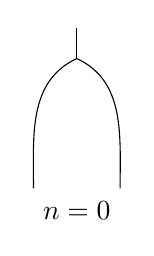
\begin{tikzpicture}[scale=.55]
		\draw (1,3.7) to (1,3); 
		
		\draw (1,3) to [out=205, in=90] (0,0);
		\draw (1,3) to [out=-25, in=90] (2,0); 
		
		\node at (1,-.5){$n=0$};
		\end{tikzpicture}\hspace*{1cm}
		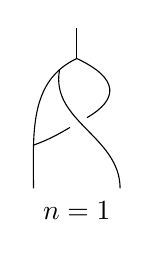
\begin{tikzpicture}[scale=.55]
		\draw (1,3.7) to (1,3); 
		
		\draw (1,3) to [out=205, in=90] (0,0);
		
		\draw [shorten >= 0cm] (.6,2.73) to [out=-100, in=90] (2,0);
		%\draw [shorten <= 0cm] (1,1.5) to [out=-60, in=90] (2,0);
		
		\draw [shorten >= .15cm] (1,3) to [out=-25, in=30, distance=1.1cm] (1,1.5);
		\draw [shorten <= .1cm] (1,1.5) to [out=210, in=20] (0,1);
		
		\node at (1,-.5){$n=1$};
		\end{tikzpicture}\hspace*{1cm}
		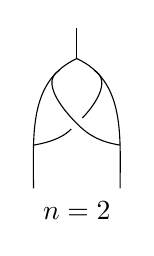
\begin{tikzpicture}[scale=.55]
		\draw (1,3.7) to (1,3); 
		
		\draw (1,3) to [out=205, in=90] (0,0);
		\draw (1,3) to [out=-25, in=90] (2,0); 
		
		\draw [shorten >= 0cm] (.6,2.73) to [out=210, in=135] (1,1.5);
		\draw [shorten <= 0cm] (1,1.5) to [out=-45, in=170] (2,1);
		
		\draw [shorten >= .1cm] (1.4,2.73) to [out=-30, in=45] (1,1.5);
		\draw [shorten <= .1cm] (1,1.5) to [out=-135, in=10] (0,1);
		
		\node at (1,-.5){$n=2$};
		\end{tikzpicture}
	}
	\caption{The values of $\psi_{U(\mathcal M)}(2)(e_n)$ for small values of $n$.}
	\label{fig: cup 0,1,2}
\end{figure}

\subsection{Cochains of simplicial sets}

In this subsection we introduce a natural May-Steenrod structure on the normalized cochains of any simplicial set $X$. Since a May-Steenrod structure was constructed in the previous section for $U(\mathcal M)$, we only need to describe a natural $U(\mathcal M)$-algebra structure on $N^\bullet(X)$. Using the linear duality functor, it suffices to construct a natural $U(\mathcal M)$-coalgebra structure on $N_\bullet(X)$ which, in turn, can be derived via a Kan extension argument from one on each $N_\bullet(\triangle^n)$. We obtain these coalgebra structures by restricting a full $\mathcal M$-bialgebra structure. An $\mathcal M$-bialgebra structure is specified by three linear maps, the images of the generators
\begin{equation*}
\counit, \quad \coproduct, \quad \product,
\end{equation*}
satisfying the relations in the presentation of $\mathcal M$. For $n \in \mathbb{N}$, define: \vspace*{5pt} \\
(1) The counit $\epsilon \in \Hom(N_\bullet(\triangle^n), \Z)$ by
\begin{equation*}
\epsilon \big( [v_0, \dots, v_q] \big) = \begin{cases} 1 & \text{ if } q = 0, \\ 0 & \text{ if } q>0. \end{cases}
\end{equation*}
(2) The coproduct $\Delta \in \Hom(N_\bullet(\triangle^n), N_\bullet(\triangle^n)^{\otimes2})$ by
\begin{equation*}
\Delta \big( [v_0, \dots, v_q] \big) = \sum_{i=0}^q [v_0, \dots, v_i] \otimes [v_i, \dots, v_q].
\end{equation*}
(3) The product $\ast \in \Hom(N_\bullet(\triangle^n)^{\otimes 2}, N_\bullet(\triangle^n))$ by
\begin{equation*}
\left[v_0, \dots, v_p \right] \ast \left[v_{p+1}, \dots, v_q\right] = \begin{cases} (-1)^{p+|\pi|} \left[v_{\pi(0)}, \dots, v_{\pi(q)}\right] & \text{ if } v_i \neq v_j \text{ for } i \neq j, \\
0 & \text{ if not}, \end{cases}
\end{equation*}
where $\pi$ is the permutation that orders the totally ordered set of vertices, and $(-1)^{|\pi|}$ its sign.

\begin{theorem} \label{thm: simplicial chain bialgebra}
	For every $n \in \mathbb{N}$, the assignment
	\begin{equation*}
	\counit \mapsto \epsilon, \quad \coproduct \mapsto \Delta, \quad \product \mapsto \ast,
	\end{equation*}
	defines a natural $\mathcal M$-bialgebra structure  on $N_\bullet(\triangle^n)$.
\end{theorem}

\begin{proof}
	This statement is proven as Theorem 4.2 in \cite{medina2020prop1}.
\end{proof}

\begin{definition}
	Let $X$ be a simplicial set. Denote by $\phi^\triangle : U(\mathcal M) \to \End_{N^\bullet (X)}$ the algebra structure obtained by dualizing the coalgebra structure induced by the restrictions of the natural $\mathcal M$-bialgebras of Theorem \ref{thm: simplicial chain bialgebra}.
\end{definition}

\begin{theorem}
	The commutative diagram
	\begin{equation*}
	\begin{tikzcd}[column sep = small, row sep = small]
	&[18pt] U(\mathcal M) \arrow[dr, "\phi^\triangle", out=0] &[-0pt] \\
	\mathcal W \arrow[ur, "\psi_{U(\mathcal M)}", in=180] \arrow[rr, "\psi^\triangle"] & & \mathrm{End}_{N^\bullet (X)}
	\end{tikzcd}
	\end{equation*}
	defines a natural May-Steenrod structure on $N^\bullet(X)$ for any simplicial set $X$.
\end{theorem}

\begin{remark}
	The $E_\infty$-structure we described in Theorem \ref{thm: simplicial chain bialgebra}, depending solely on three fundamental maps, recovers the coalgebra structures of McClure-Smith \cite{mcclure03cochain} and, up to signs, that of Berger-Fresse \cite{berger04combinatorial}.
\end{remark}

\begin{example}
	Let us consider the prime $2$. The value $P^1(x)\big([0,1,2,3,4]\big)$ for a homogeneous cocycle $x$ in $N^{-3}(\triangle^4)$ is equal to the value of $x^{\otimes 2}$ acting on
	\begin{align*}
	[0, 1, 2, 3] \otimes [0, 1, 3, 4] \ +\  & 
	[0, 2, 3, 4] \otimes [0, 1, 2, 4] \\ \ +\ 
	[0, 1, 2, 3] \otimes [1, 2, 3, 4] \ +\ &
	[0, 1, 3, 4] \otimes [1, 2, 3, 4].
	\end{align*}
	Similarly, the value of $P^2(y)\big([0,1,2,3,4,5,6,7]\big)$ for a homogeneous cocycle $y$ in $N^{-5}(\triangle^7)$ is equal to the value of $y^{\otimes 2}$ acting on
	\begin{align*}
	[0, 1, 2, 5, 6, 7] \otimes [0, 1, 2, 3, 4, 5] & \ +\
	[0, 1, 2, 3, 6, 7] \otimes [0, 1, 3, 4, 5, 6] \\ \ +\ 
	[0, 1, 2, 3, 4, 7] \otimes [0, 1, 4, 5, 6, 7] & \ +\ 
	[0, 2, 3, 5, 6, 7] \otimes [0, 1, 2, 3, 4, 5] \\ \ +\ 
	[0, 2, 3, 4, 6, 7] \otimes [0, 1, 2, 4, 5, 6] & \ +\ 
	[0, 2, 3, 4, 5, 7] \otimes [0, 1, 2, 5, 6, 7] \\ \ +\ 
	[0, 3, 4, 5, 6, 7] \otimes [0, 1, 2, 3, 4, 5] & \ +\ 
	[0, 3, 4, 5, 6, 7] \otimes [0, 1, 2, 3, 5, 6] \\ \ +\ 
	[0, 3, 4, 5, 6, 7] \otimes [0, 1, 2, 3, 6, 7] & \ +\ 
	[0, 1, 2, 3, 6, 7] \otimes [1, 2, 3, 4, 5, 6] \\ \ +\ 
	[0, 1, 2, 3, 4, 7] \otimes [1, 2, 4, 5, 6, 7] & \ +\ 
	[0, 1, 3, 4, 6, 7] \otimes [1, 2, 3, 4, 5, 6] \\ \ +\ 
	[0, 1, 3, 4, 5, 7] \otimes [1, 2, 3, 5, 6, 7] & \ +\ 
	[0, 1, 4, 5, 6, 7] \otimes [1, 2, 3, 4, 5, 6] \\ \ +\ 
	[0, 1, 4, 5, 6, 7] \otimes [1, 2, 3, 4, 6, 7] & \ +\ 
	[0, 1, 2, 3, 4, 7] \otimes [2, 3, 4, 5, 6, 7] \\ \ +\ 
	[0, 1, 2, 4, 5, 7] \otimes [2, 3, 4, 5, 6, 7] & \ +\ 
	[0, 1, 2, 5, 6, 7] \otimes [2, 3, 4, 5, 6, 7].
	\end{align*}
\end{example}

\begin{example}
	Let us consider the prime $3$. The value $\beta P^1(x)\big([0,1,2,3,4,5,6,7,8]\big)$ for a homogeneous cocycle $x$ in $N^{-3}(\triangle^8)$ is equal to the value of $x^{\otimes 3}$ acting on
	\begin{align*}
	& \,-\, [0, 6, 7, 8] \otimes [0, 1, 2, 3] \otimes [3, 4, 5, 6] \,+\, [0, 1, 7, 8] \otimes [1, 2, 3, 4] \otimes [4, 5, 6, 7] \\ & \,-\, [0, 1, 2, 8] \otimes [2, 3, 4, 5] \otimes [5, 6, 7, 8].
	\end{align*}
	Similarly, the value of $P^1(y)\big([0,1,\dots,7]\big)$ for a homogeneous cocycle $y$ in $N^{-3}(\triangle^7)$ is equal to the value of $y^{\otimes 3}$ acting on
	\begin{align*}
	& \,-\, [0,3,4,5] \otimes [0,5,6,7] \otimes [0,1,2,3] \,-\, [0,4,5,6] \otimes [0,1,6,7] \otimes [1,2,3,4] \\ & \,-\, [0,5,6,7] \otimes [0,1,2,7] \otimes [2,3,4,5] \,-\, [0,1,4,5] \otimes [1,5,6,7] \otimes [1,2,3,4] \\ & \,+\, [0,1,5,6] \otimes [1,2,6,7] \otimes [2,3,4,5] \,-\, [0,1,6,7] \otimes [1,2,3,7] \otimes [3,4,5,6] \\ & \,-\, [0,1,2,5] \otimes [2,5,6,7] \otimes [2,3,4,5] \,-\, [0,1,2,6] \otimes [2,3,6,7] \otimes [3,4,5,6] \\ & \,-\, [0,1,2,7] \otimes [2,3,4,7] \otimes [4,5,6,7] \,+\, [0,1,2,3] \otimes [3,4,5,6] \otimes [0,1,6,7] \\ & \,+\, [0,2,3,4] \otimes [4,5,6,7] \otimes [0,1,2,7] \,+\, [0,1,2,3] \otimes [3,4,5,6] \otimes [1,2,6,7] \\ & \,-\, [0,1,3,4] \otimes [4,5,6,7] \otimes [1,2,3,7] \,+\, [0,1,2,3] \otimes [3,4,5,6] \otimes [2,3,6,7] \\ & \,+\, [0,1,2,4] \otimes [4,5,6,7] \otimes [2,3,4,7] \,+\, [0,1,2,3] \otimes [3,4,5,6] \otimes [3,4,6,7] \\ & \,-\, [0,1,2,3] \otimes [3,5,6,7] \otimes [3,4,5,7] \,+\, [0,1,2,3] \otimes [3,4,5,6] \otimes [4,5,6,7] \\ & \,+\, [0,1,2,3] \otimes [3,4,6,7] \otimes [4,5,6,7].
	\end{align*}
\end{example}

\subsection{Cochains of cubical sets}

In this subsection we introduce a natural May-Steenrod structure on the normalized cochains of any cubical set. It follows the structure of the previous subsection closely. By the same considerations, the desired construction will follow from a natural $\mathcal M$-bialgebra structure on $N_\bullet(\square^n)$. These are determined by three linear maps satisfying the relations in the presentation of $\mathcal M$. For $n \in \mathbb{N}$, define: \vspace*{5pt} \\
(1) The counit $\epsilon \in \Hom(N_\bullet(\square^n), \Z)$ by
\begin{equation*}
\epsilon \left( x_1 \otimes \cdots \otimes x_d \right) = \epsilon(x_1) \cdots \, \epsilon(x_n),
\end{equation*}
where
\begin{equation*}
\epsilon([0]) = \epsilon([1]) = 1, \qquad \epsilon([0, 1]) = 0.
\end{equation*} \vspace*{-6pt} \\
(2) The coproduct $\Delta \in \Hom \left( N_\bullet(\square^n), N_\bullet(\square^n)^{\otimes 2} \right)$ by
\begin{equation*}	
\Delta (x_1 \otimes \cdots \otimes x_n) = 	
\sum \pm \left( x_1^{(1)} \otimes \cdots \otimes x_n^{(1)} \right) \otimes 	
\left( x_1^{(2)} \otimes \cdots \otimes x_n^{(2)} \right),	
\end{equation*}	
where the sign is determined using the Koszul convention, and we are using Sweedler's notation
\begin{equation*}	
\Delta(x_i) = \sum x_i^{(1)} \otimes x_i^{(2)}
\end{equation*}
for the chain map $\Delta \colon N_\bullet(\square^1) \to N_\bullet(\square^1)^{\otimes 2}$ defined by
\begin{equation*}
\Delta([0]) = [0] \otimes [0], \quad \Delta([1]) = [1] \otimes [1], \quad \Delta([0, 1]) = [0] \otimes [0, 1] + [0, 1] \otimes [1].
\end{equation*}
Using that $N_\bullet(\square^n) = N_\bullet(\square^1)^{\otimes n}$, $\Delta$ is the composition
\begin{equation*}
\begin{tikzcd}
N_\bullet(\square^1)^{\otimes n} \arrow[r, "\Delta^{\otimes n}"] & \left( N_\bullet(\square^1)^{\otimes 2}  \right)^{\otimes n} \arrow[r, "sh"] & \left( N_\bullet(\square^1)^{\otimes n} \right)^{\otimes 2}
\end{tikzcd}
\end{equation*}
where $sh$ is the shuffle map that places tensor factors in odd position first. \vspace*{5pt} \\
(3) The product $\ast \in \Hom(N_\bullet(\square^n)^{\otimes 2}, N_\bullet(\square^n))$ by
\begin{align*}
(x_1 \otimes \cdots \otimes x_n) \ast (y_1 \otimes \cdots \otimes y_n) =
(-1)^{|x|} \sum_{i=1}^n x_{<i} \epsilon(y_{<i}) \otimes x_i \ast y_i \otimes \epsilon(x_{>i})y_{>i},
\end{align*}
where
\begin{align*}
x_{<i} & = x_1 \otimes \cdots \otimes x_{i-1}, &
y_{<i} & = y_1 \otimes \cdots \otimes y_{i-1}, \\
x_{>i} & = x_{i+1} \otimes \cdots \otimes x_n, & 
y_{>i} & = y_{i+1} \otimes \cdots \otimes y_n,
\end{align*}
with the convention
\begin{equation*}
x_{<1} = y_{<1} = x_{>n} = y_{>n} = 1 \in \Z,
\end{equation*}
and the only non-zero values of $x_i \ast y_i$ are
\begin{equation*}
\ast([0] \otimes [1]) = [0, 1], \qquad  \ast([1] \otimes [0]) = -[0, 1].
\end{equation*}

\begin{theorem} \label{thm: cubical chain bialgebra}
	For every $n \in \mathbb{N}$, the assignment
	\begin{equation*}
	\counit \mapsto \epsilon, \quad \coproduct \mapsto \Delta, \quad \product \mapsto \ast,
	\end{equation*}
	defines a natural $\mathcal M$-bialgebra structure on $N_\bullet(\square^n)$.
\end{theorem}

\begin{proof}
	We present a proof of this statement in the appendix.
\end{proof}

\begin{remark}
	We saw that for simplicial sets a natural algebraic $E_\infty$-structure was determined by basic maps in the standard simplices. For cubical sets, one such structure is constructed by naturally extending three maps defined just on the interval. 
\end{remark}

\begin{definition}
	Let $X$ be a cubical set. Denote by $\phi^\square : U(\mathcal M) \to \End_{N^\bullet (X)}$ the algebra structure obtained by dualizing the coalgebra structure induced by the restrictions of the natural $\mathcal M$-bialgebras of Theorem~\ref{thm: cubical chain bialgebra}.
\end{definition}

\begin{theorem}
	The commutative diagram
	\begin{equation*}
	\begin{tikzcd}[column sep = small, row sep = small]
	&[18pt] U(\mathcal M) \arrow[dr, "\phi^\square", out=0] &[-0pt] \\
	\mathcal W \arrow[ur, "\psi_{U(\mathcal M)}", in=180] \arrow[rr, "\psi^\square"] & & \End_{N^\bullet (X)}
	\end{tikzcd}
	\end{equation*}
	defines a natural May-Steenrod structure on $N^\bullet(X)$ for any cubical set $X$.
\end{theorem}

\begin{example}
	Let us consider the prime $2$. The value $P^1(x)\big([01]^{4}\big)$ for a homogeneous cocycle $x$ in $N^{-3}(\square^4)$ is equal to the value of $x^{\otimes 2}$ acting on
	\begin{align*}&
	[01]1[01][01] \otimes [01][01]0[01]\,+\,
	[01][01][01]0 \otimes [01]0[01][01]\,+\, \\&
	[01][01][01]0 \otimes 1[01][01][01]\,+\,
	[01][01]1[01] \otimes [01]0[01][01]\,+\, \\&
	[01][01]1[01] \otimes 1[01][01][01]\,+\,
	[01][01][01]0 \otimes [01][01]1[01]\,+\, \\&
	[01][01]0[01] \otimes [01][01][01]1\,+\,
	[01]1[01][01] \otimes [01][01][01]1\,+\, \\&
	0[01][01][01] \otimes [01][01][01]1\,+\,
	0[01][01][01] \otimes [01][01]0[01]\,+\, \\&
	0[01][01][01] \otimes [01]1[01][01]\,+\,
	[01]0[01][01] \otimes 1[01][01][01].\,\phantom{+}\,
	\end{align*}
\end{example}

\begin{example}
	Let us consider the prime $3$. The value of $\beta P^0(x)\big([01]^2\big)$ for a homogeneous cocycle $x$ in $N^{-1}(\square^2)$ is equal to the value of $x^{\otimes 3}$ acting on
	\begin{align*}
	\,-\, [01]1 \otimes [01]0 \otimes 1[01] \,-\, 0[01] \otimes [01]0 \otimes 1[01] + [01]1 \otimes 0[01] \otimes [01]1 + 0[01] \otimes 0[01] \otimes [01]1.
	\end{align*}
\end{example}

